
% General typesetting
%\newcommand{\toolfont}[1]{\texttt{#1}}
\newcommand{\toolfont}[1]{{#1}}
\newcommand{\newparagraph}{\par\nopagebreak\bigskip\nopagebreak\noindent}
%\newcommand{\arxivlink}[1]{\href{http://arxiv.org/abs/#1}{\texttt{arXiv:#1}}}
\newcommand{\arxivlink}[1]{\href{http://arxiv.org/abs/#1}{arXiv:#1}}
% \newcommand{\comment}[1]{\marginpar{\sffamily\footnotesize\textcolor{dark-red}{#1}}}
% \newcommand{\comment}[1]{} % for proof readers

% General symbols 
\newcommand{\im}{\mathrm{i}}
\newcommand{\diff}{\mathrm{d}}
\newcommand{\eg}{{e.\,g.}~}
\newcommand{\ie}{{i.\,e.}~}
\newcommand{\largex}{{\large \ensuremath{\boldsymbol{\times}}}}
\newcommand{\brlargex}{{\large \ensuremath{(\boldsymbol{\times})}}}
\newcommand{\equivalent}{\simeq}

% Spaces
\newcommand{\qqquad}{\qquad \qquad}
\newcommand{\qqqquad}{\qqquad \qqquad}
\newcommand{\qqqqquad}{\qqqquad \qqqquad}

% Physics symbols
\newcommand{\mat}[1]{\mathcal{M}_\text{#1}}
\newcommand{\lgr}[1]{\mathcal{L}_\text{#1}}
\newcommand{\ord}[1]{\mathcal{O}\left(#1\right)}
\newcommand{\br}{\mathrm{BR}}
\newcommand{\mpt}{{\ensuremath{\mathbf{p}_T^{\text{miss}}}}}
%\newcommand{\met}{\ensuremath{\slashed{E}_T}}
\newcommand{\met}{{\ensuremath{E_T^{\text{miss}}}}}
\newcommand{\phisq}{\phi^\dagger \phi}
\newcommand{\seff}{S_{\text{eff}}}

% Operators 
\newcommand{\ope}[1]{\mathcal{O}_{#1}}
\newcommand{\opesilh}[1]{\mathcal{O}_{#1}^{\text{SILH}}}
\newcommand{\opeother}[1]{\mathcal{O}'_{#1}}

% Units
%\newcommand{\ifb}{\ensuremath \mathrm{fb}^{-1}}
%\newcommand{\gev}{{\ensuremath \mathrm{GeV}}}
%\newcommand{\tev}{{\ensuremath \mathrm{TeV}}}
\newcommand{\ev}{\si{eV}}
\newcommand{\kev}{\si{keV}}
\newcommand{\mev}{\si{MeV}}
\newcommand{\gev}{\si{GeV}}
\newcommand{\tev}{\si{TeV}}
\newcommand{\fb}{\si{fb}}
\newcommand{\ifb}{\si{fb^{-1}}}
\newcommand{\pb}{\si{pb}}
\newcommand{\ipb}{\si{pb^{-1}}}

% Derivatives and commutators
\newcommand{\pder}[2]{\frac {\partial #1} {\partial #2}}
\newcommand{\tder}[2]{\frac {\diff #1} {\diff #2}}
\newcommand{\ttder}[2]{\frac {\diff^2 #1} {\diff {#2}^2}}
\newcommand{\fder}[2]{\frac {\delta #1} {\delta #2}}
\newcommand{\cmt}[2]{\left[ #1 , #2 \right]}
\newcommand{\acmt}[2]{\left\{ #1 , #2 \right\}}

% Integrals
\newcommand{\intx}{\int \!\! \mathrm{d} x\;}
\newcommand{\intxprime}{\int \!\! \mathrm{d} x'\;}
\newcommand{\intxi}{\int \!\! \mathrm{d} x_i\;}
\newcommand{\intxk}{\int \!\! \mathrm{d} x_k\;}
\newcommand{\intfatx}{\int \!\! \mathrm{d} \mathbf{x}\;}

\newcommand{\intthreex}{\int \!\! \mathrm{d}^3 x\;}
\newcommand{\intfourx}{\int \!\! \mathrm{d}^4 x\;}
\newcommand{\intfoury}{\int \!\! \mathrm{d}^4 y\;}
\newcommand{\intfourz}{\int \!\! \mathrm{d}^4 z\;}

\newcommand{\intthreek}{\int \!\! \frac {\mathrm{d}^3 k} {(2\pi)^3}\;}
\newcommand{\intfourk}{\int \!\! \frac {\mathrm{d}^4 k} {(2\pi)^4}\;}
\newcommand{\intfourke}{\int \!\! \frac {\mathrm{d}^4 k_E} {(2\pi)^4}\;}
\newcommand{\intthreep}{\int \!\! \frac {\mathrm{d}^3 p} {(2\pi)^3}\;}
\newcommand{\intfourp}{\int \!\! \frac {\mathrm{d}^4 p} {(2\pi)^4}\;}
\newcommand{\intfourq}{\int \!\! \frac {\mathrm{d}^4 q} {(2\pi)^4}\;}

\newcommand{\intfatthetahat}{\int \!\! \mathrm{d} \hat{\boldtheta}\;}

% Vectors
\newcommand{\twovec}[2]{\begin{pmatrix*}[c] #1 \\ #2 \end{pmatrix*}}
\newcommand{\threevec}[3]{\begin{pmatrix*}[c] #1 \\ #2 \\ #3\end{pmatrix*}}
\newcommand{\fourvec}[4]{\begin{pmatrix*}[c] #1 \\ #2 \\ #3 \\ #4 \end{pmatrix*}}
\newcommand{\fivevec}[5]{\begin{pmatrix*}[c] #1 \\ #2 \\ #3 \\ #4 \\ #5 \end{pmatrix*}}

\newcommand{\fourvecr}[4]{\begin{pmatrix*}[r] #1 \\ #2 \\ #3 \\ #4 \end{pmatrix*}}
\newcommand{\fivevecr}[5]{\begin{pmatrix*}[r] #1 \\ #2 \\ #3 \\ #4 \\ #5 \end{pmatrix*}}
\newcommand{\sixvecr}[6]{\begin{pmatrix*}[r] #1 \\ #2 \\ #3 \\ #4 \\ #5 \\ #6 \end{pmatrix*}}
\newcommand{\eightvecr}[8]{\begin{pmatrix*}[r] #1 \\ #2 \\ #3 \\ #4 \\ #5 \\ #6 \\ #7 \\ #8 \end{pmatrix*}}

% Matrices 
\newcommand{\twomat}[4]{\begin{pmatrix*}[c] #1 & #2\\ #3 & #4 \end{pmatrix*}}
\newcommand{\threemat}[9]{\begin{pmatrix*}[c] #1 & #2 & #3\\ #4 & #5 & #6 \\ #7 & #8 & #9\end{pmatrix*}}

\newcommand{\twomatr}[4]{\begin{pmatrix*}[r] #1 & #2\\ #3 & #4 \end{pmatrix*}}
\newcommand{\threematr}[9]{\begin{pmatrix*}[r] #1 & #2 & #3\\ #4 & #5 & #6 \\ #7 & #8 & #9\end{pmatrix*}}

% Bold symbols
\newcommand{\boldtheta}{{\ensuremath \boldsymbol{\theta}}}
\newcommand{\boldnu}{\ensuremath \boldsymbol{\nu}}
\newcommand{\boldepsilon}{\ensuremath \boldsymbol{\varepsilon}}
\newcommand{\boldx}{\ensuremath \mathbf{x}}
\newcommand{\boldv}{\ensuremath \mathbf{v}}
\newcommand{\boldzero}{\ensuremath \mathbf{0}}

% Distance definitions
\newcommand{\dlocal}{d_{\text{local}}}

% Column types
\newcolumntype{R}{>{\raggedleft\arraybackslash}X}%
\newcolumntype{L}{>{\raggedright\arraybackslash}X}%

% feynmp momentum arrows:
% \marrow{name}{arrow_pos}{text_pos}{text}{nodes}
% name: no numbers
% arrow_pos: up, down, left, right
% text_pos: top, bot, lft, rt
\newcommand{\marrow}[5]{%
    \fmfcmd{style_def marrow#1
    expr p = drawarrow subpath (1/4, 3/4) of p shifted 6 #2 withpen pencircle scaled 0.4;
    label.#3(btex #4 etex, point 0.5 of p shifted 6 #2);
    enddef;}
    \fmf{marrow#1,tension=0}{#5}}

% Longer \bar
\newcommand{\overbar}[1]{\mkern 1.5mu\overline{\mkern-1.5mu#1\mkern-1.5mu}\mkern 1.5mu}

% includegraphics with default dummy
%\newcommand{\includegraphicsdummy}[2][{}]{\IfFileExists{#2}{\includegraphics[#1]{#2}}{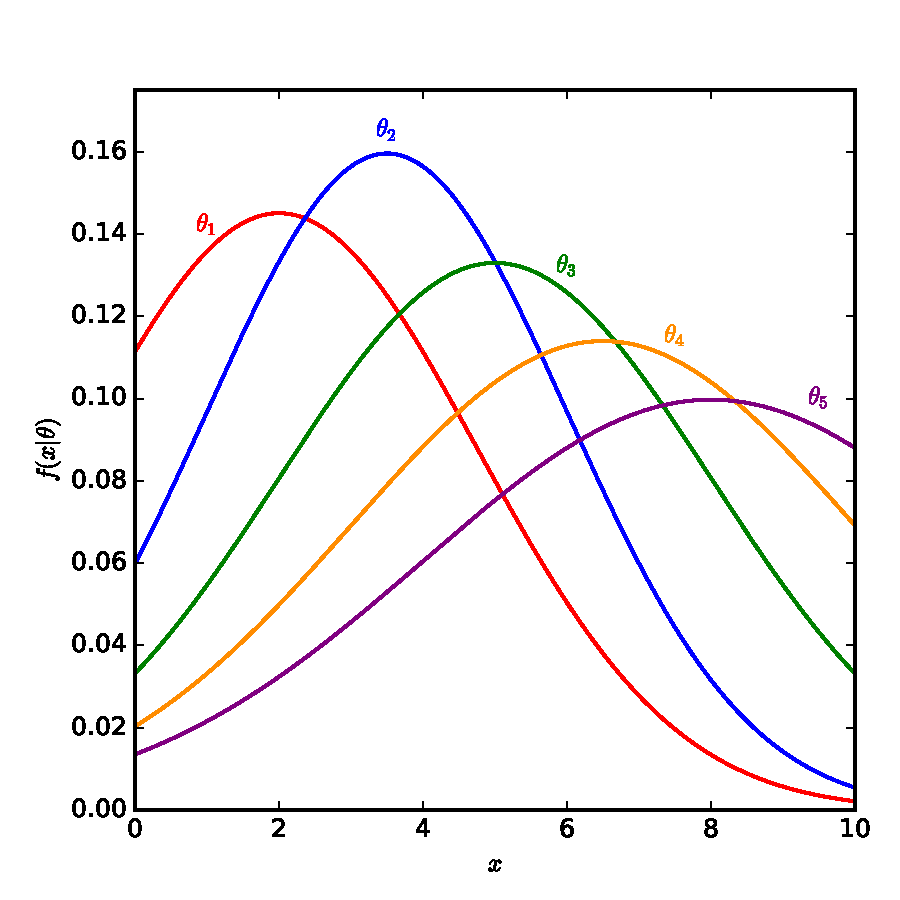
\includegraphics[#1]{fig/general/dummy.pdf}}}

% Math operators
\DeclareMathOperator{\tr}{tr}
\DeclareMathOperator{\Tr}{Tr}
\DeclareMathOperator{\diag}{diag}
\DeclareMathOperator{\Real}{Re}
\DeclareMathOperator{\Pois}{Pois}
\DeclareMathOperator{\cov}{cov}
\DeclareMathOperator{\var}{var}
\DeclareMathOperator{\BR}{BR}
\DeclareMathOperator{\hc}{h.\,c.}
\DeclareMathOperator*{\argmax}{arg\,max}

% Title page
\newcommand{\tptitle}[1]{{\Huge \sffamily \bfseries #1 }}
\newcommand{\tpauthor}[1]{{\LARGE \rmfamily #1 }}
\newcommand{\tplarge}[1]{{\large \rmfamily #1 }}
\newcommand{\tpsmall}[1]{{\rmfamily #1 }}
\newcommand{\tpskip}{\vspace*{0.18cm}}
\newcommand{\tpbigskip}{\vspace*{0.3cm}}

% Capitals at beginning of chapter
\newcommand{\firstword}[2]{\lettrine[lines=3]{\color{highlight-color}#1}{#2}}

% feynmf
\newcommand{\feynmansetup}{%
      \fmfpen{0.8pt}%
      \fmfset{arrow_len}{2mm}%
}

% Very specific things for this thesis
\newcommand{\wbfpyramid}[3]{%
\begin{figure}
%trimming options: L B R T
  \includegraphics[height=0.225 \textwidth,clip=true,trim=0.cm 1.9cm 2.48cm 0.1cm]{fig/information/#1_fw_fb.pdf}\,%
  \phantom{\includegraphics[height=0.225 \textwidth,clip=true,trim=1.9cm 1.9cm 2.48cm 0.1cm]{fig/information/#1_fww_fw.pdf}}\,%
  \phantom{\includegraphics[height=0.225 \textwidth,clip=true,trim=1.9cm 1.9cm 2.48cm 0.1cm]{fig/information/#1_fww_fw.pdf}}\,%
  \phantom{\includegraphics[height=0.225 \textwidth,clip=true,trim=1.9cm 1.9cm 0.3cm 0.1cm]{fig/information/#1_fww_fw.pdf}}\\%
%
  \includegraphics[height=0.225 \textwidth,clip=true,trim=0.cm 1.9cm 2.48cm 0.1cm]{fig/information/#1_fbb_fb.pdf}\,%
  \includegraphics[height=0.225 \textwidth,clip=true,trim=1.9cm 1.9cm 2.48cm 0.1cm]{fig/information/#1_fbb_fw.pdf}\,%
  \phantom{\includegraphics[height=0.225 \textwidth,clip=true,trim=1.9cm 1.9cm 2.48cm 0.1cm]{fig/information/#1_fww_fw.pdf}}\,%
  \phantom{\includegraphics[height=0.225 \textwidth,clip=true,trim=1.9cm 1.9cm 0.3cm 0.1cm]{fig/information/#1_fww_fw.pdf}}\\%
%
  \includegraphics[height=0.225 \textwidth,clip=true,trim=0.cm 1.9cm 2.48cm 0.1cm]{fig/information/#1_fww_fb.pdf}\,%
  \includegraphics[height=0.225 \textwidth,clip=true,trim=1.9cm 1.9cm 2.48cm 0.1cm]{fig/information/#1_fww_fw.pdf}\,%
  \includegraphics[height=0.225 \textwidth,clip=true,trim=1.9cm 1.9cm 2.48cm 0.1cm]{fig/information/#1_fww_fbb.pdf}\,%
  \phantom{\includegraphics[height=0.225 \textwidth,clip=true,trim=1.9cm 1.9cm 0.3cm 0.1cm]{fig/information/#1_fww_fw.pdf}}\\%
%
  \includegraphics[height=0.2633 \textwidth,clip=true,trim=0.cm 0.3cm 2.48cm 0.1cm]{fig/information/#1_fphi2_fb.pdf}\,%
  \includegraphics[height=0.2633 \textwidth,clip=true,trim=1.9cm 0.3cm 2.48cm 0.1cm]{fig/information/#1_fphi2_fw.pdf}\,%
  \includegraphics[height=0.2633 \textwidth,clip=true,trim=1.9cm 0.3cm  2.48cm 0.1cm]{fig/information/#1_fphi2_fbb.pdf}\,%
  \includegraphics[height=0.2633 \textwidth,clip=true,trim=1.9cm 0.3cm  0.3cm 0.1cm]{fig/information/#1_fphi2_fww.pdf}%
  \caption{#3}
  \label{#2}
\end{figure}
}

\newcommand{\thpyramid}[3]{%
\begin{figure}
%trimming options: L B R T
  \includegraphics[height=0.29 \textwidth,clip=true,trim=0.3cm 1.9cm 2.48cm 0.1cm]{fig/information/#1_fww_fw.pdf}\,%
  \phantom{\includegraphics[height=0.29  \textwidth,clip=true,trim=1.9cm 1.9cm 2.48cm 0.1cm]{fig/information/#1_fww_fw.pdf}}\,%
  \phantom{\includegraphics[height=0.29  \textwidth,clip=true,trim=1.9cm 1.9cm 0.3cm 0.1cm]{fig/information/#1_fww_fw.pdf}}\\%
%
  \includegraphics[height=0.29 \textwidth,clip=true,trim=0.3cm 1.9cm 2.48cm 0.1cm]{fig/information/#1_ft_fw.pdf}\,%
  \includegraphics[height=0.29 \textwidth,clip=true,trim=1.9cm 1.9cm 2.48cm 0.1cm]{fig/information/#1_ft_fww.pdf}\,%
  \phantom{\includegraphics[height=0.29 \textwidth,clip=true,trim=1.9cm 1.9cm 0.3cm 0.1cm]{fig/information/#1_fww_fw.pdf}}\\%
%
  \includegraphics[height=0.33 \textwidth,clip=true,trim=0.3cm 0.6cm 2.48cm 0.1cm]{fig/information/#1_fphi2_fw.pdf}\,%
  \includegraphics[height=0.33 \textwidth,clip=true,trim=1.9cm 0.6cm 2.48cm 0.1cm]{fig/information/#1_fphi2_fww.pdf}\,%
  \includegraphics[height=0.33 \textwidth,clip=true,trim=1.9cm 0.6cm 0.3cm 0.1cm]{fig/information/#1_fphi2_ft.pdf}%
  \caption{#3}
  \label{#2}
\end{figure}
}